%************************************************
\chapter{Sonometer}
%************************************************
\begin{flushright}
October 9, 10 2012
\end{flushright}
\section{Aim}
	To 
	\begin{enumerate}
		\item observe standing waves in a streteched string
		\item vary length and linear density of the sonometer wire and observe changes in frequency
		\item find linear density of an unknown wire
		\item find the fundamental modes using an AC source
	\end{enumerate}

	\section{Apparatus}
	Sonometer, Tuning Forks, Weights, Weighing Machine, Screw Gauge, Magnetic Coil and appropriate circuitry

\section{Theory}
	This experiment is based on a single formula which is
	\begin{equation}
		f=n\frac{v}{\lambda}=n\frac{1}{2l}\sqrt{\frac{T}{m}}
	\end{equation}
	where $f$ is the frequency, $n$ represents the mode of vibration, $l$ is length of the wire, $T$ is the tension on the wire and $m$ is mass per unit length of the wire. The only caveat here is to understand that $f_{ac}$ actually excites the string with twice the frequency because it attracts at both times, producing a $2f_{ac}$ frequency in the wire.
	\par
	We keep, for the first experiment, tension and the wire constant, and find the first fundamental mode for various frequencies. We repeat this for the other wire. The slope of the frequency against fundamental length inverse graph will yield
	\begin{equation}
		m_{line}=lf=\frac{1}{2}\sqrt{\frac{T}{m}}
	\end{equation}
	This was used to find the mass per unit length, since the Tension is already known.	
	\par
	For the next part, the frequency was taken from the AC source, and length of string was plotted against $n$. The slope of the graph yields
	\begin{equation}
		m_{line}=\frac{l}{n}=\frac{1}{2f}\sqrt{\frac{T}{m}}
	\end{equation}
	where $f$ and $T$ are again known, and $m$ was determined using the slope.

\section{Procedure}
	\begin{enumerate}
		\item Tension and effective length of steel wire were varied and fundamental modes of frequencies were obtained for these values. 
		\item The mass per unit length of the wire was calculated as described in the theory. From the slope of best fit line for the plot of frequency f vs 1/L, value of fL can be calculated.
		\item The experiment was repeated for brass wire.
		\item With the steel wire, given L, T and frequency of a magnetic vibrator, the mass per unit length can again be calculated. If the magnetic vibrator is placed above the wire and length L is gradually changed, the frequency of the wire at which it vibrated with the maximum amplitude is the frequency of the oscillator.
	\end{enumerate}
	
\section{Result and Observations}
	The observations are given in \autoref{4_brass} and for the Steel Wire are given in \autoref{4_steel}. The AC source observations are given in \autoref{4_steel2}. In accordance with these, the mass per unit length of the brass wire was found out to be $38.4 \pm 1.9 mg/cm$. For the steel wire, using the Tuning Fork method, the value was found out to be $33.8 \pm 1.9 mg/cm$ and using the AC method, this turned out to be $552 \pm 79 mg/cm$. This may be explained by realizing that the first fundamental length was missed in the Tuning Fork experiment.
	\begin{figure}[bth]
		\begin{center}
			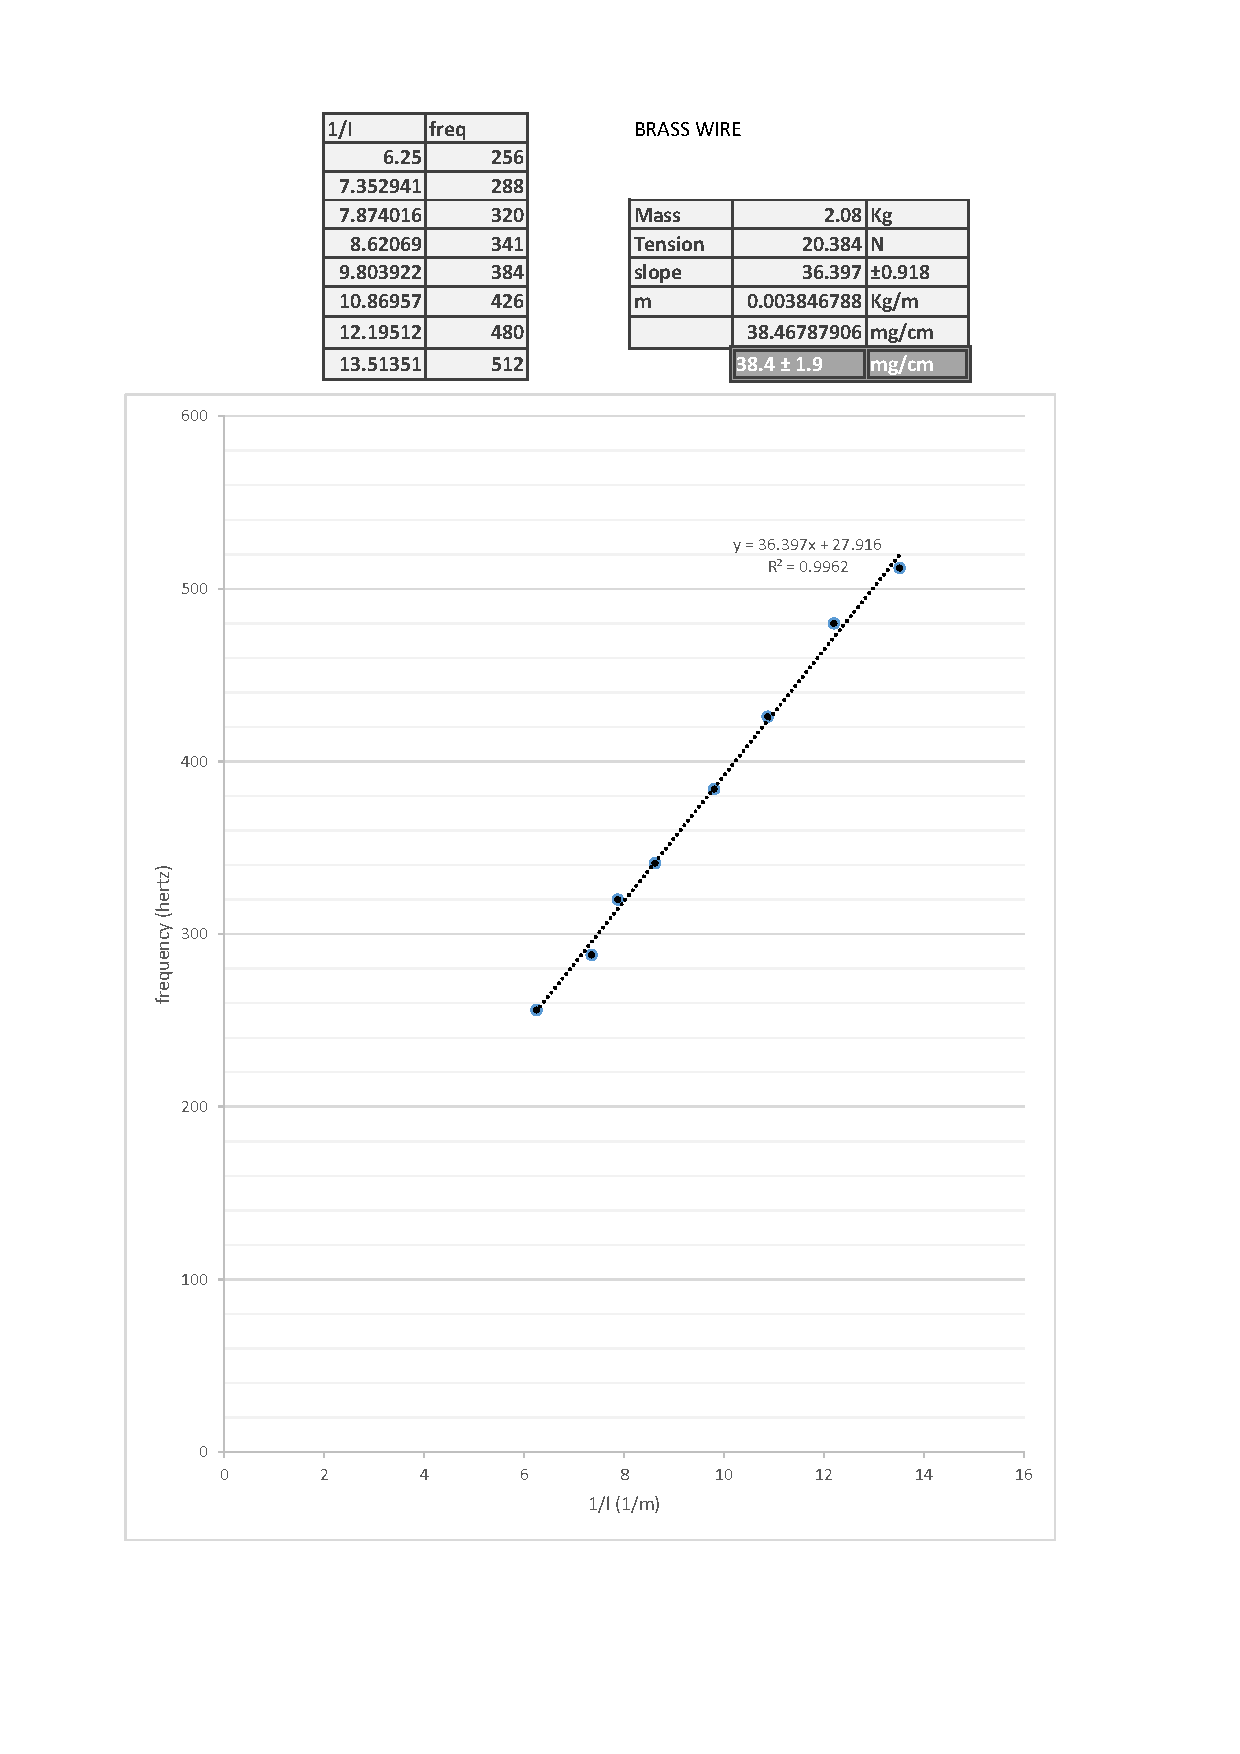
\includegraphics[width=1.3\linewidth]{gfx/brass}
		\end{center}
		\caption[Brass Wire]{Brass Wire}
	\label{4_brass}
	\end{figure}

	\begin{figure}[bth]
		\begin{center}
			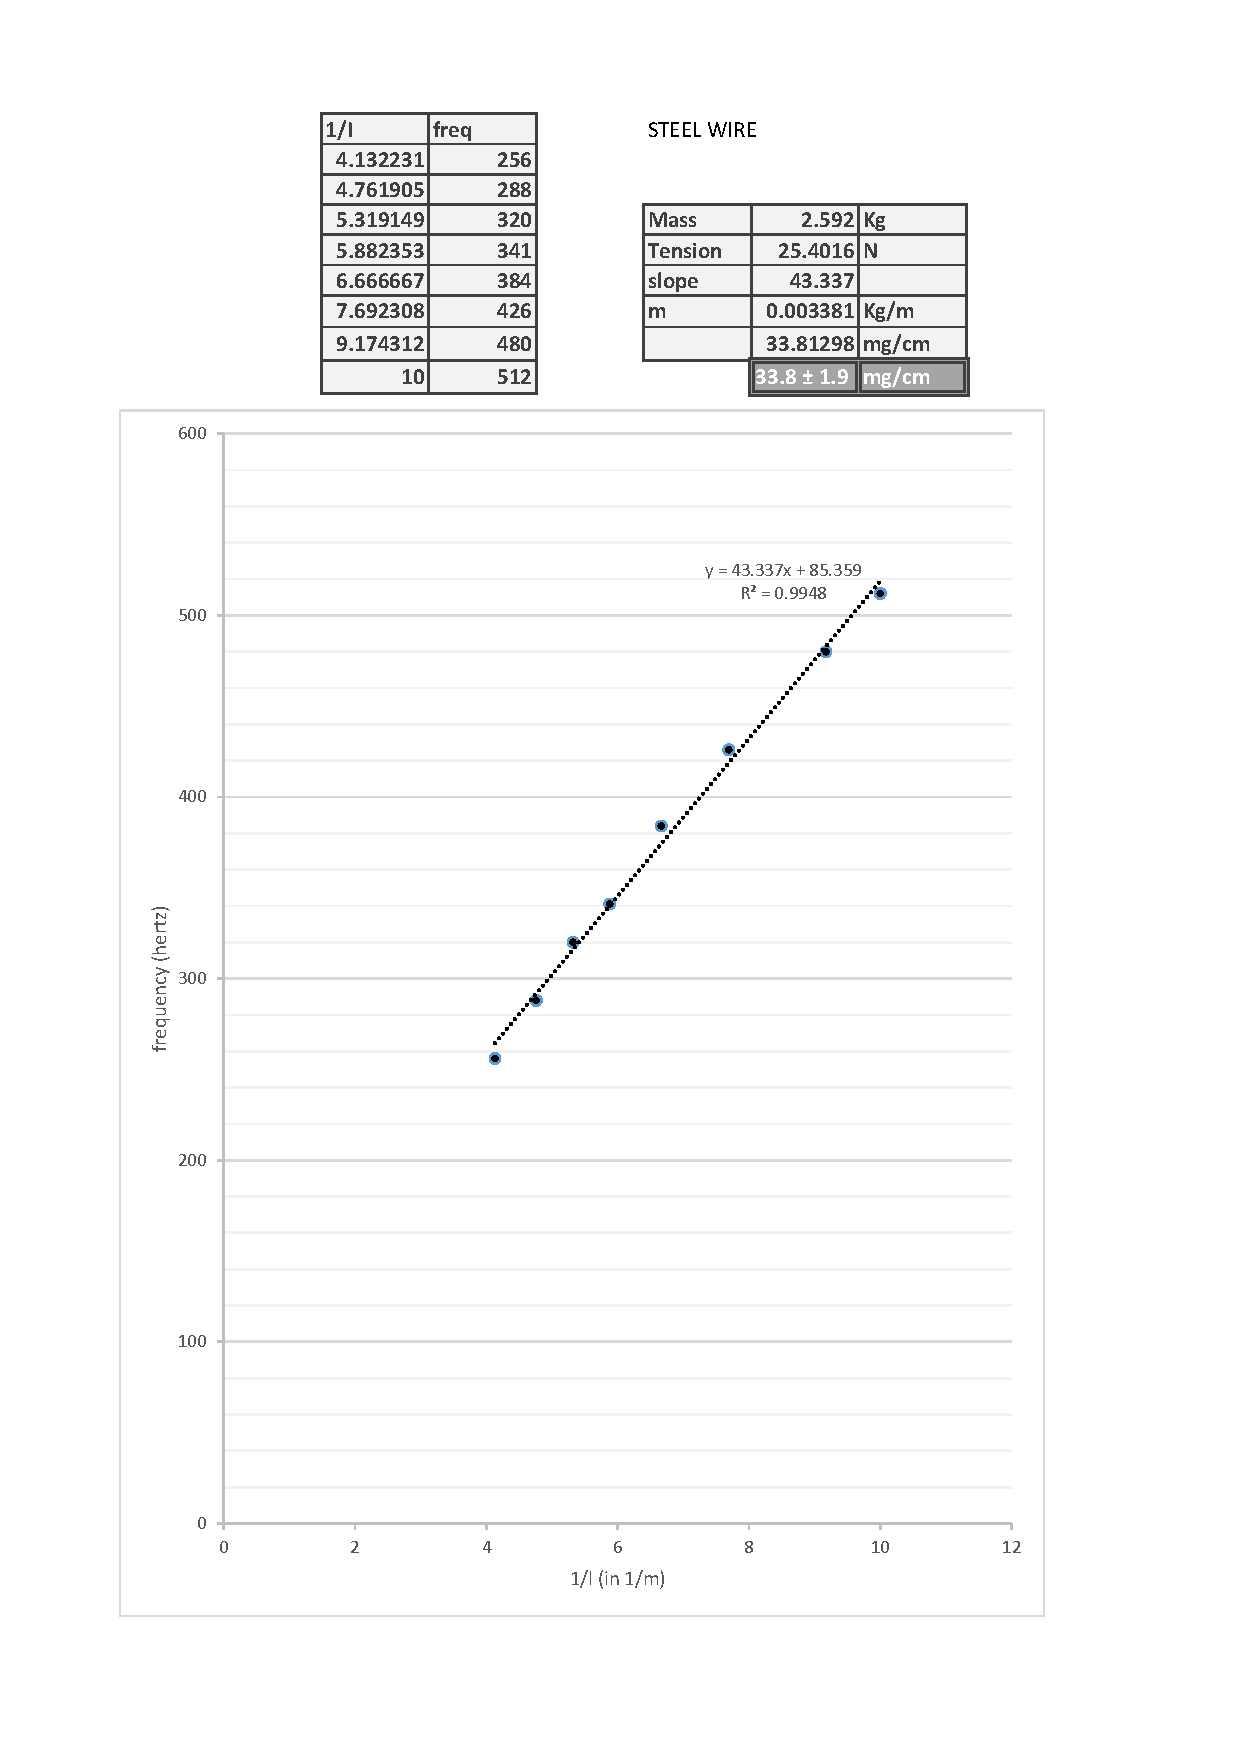
\includegraphics[width=1.3\linewidth]{gfx/steel}
		\end{center}
		\caption[Brass Wire]{Brass Wire}
	\label{4_steel}
	\end{figure}

	\begin{figure}[bth]
		\begin{center}
			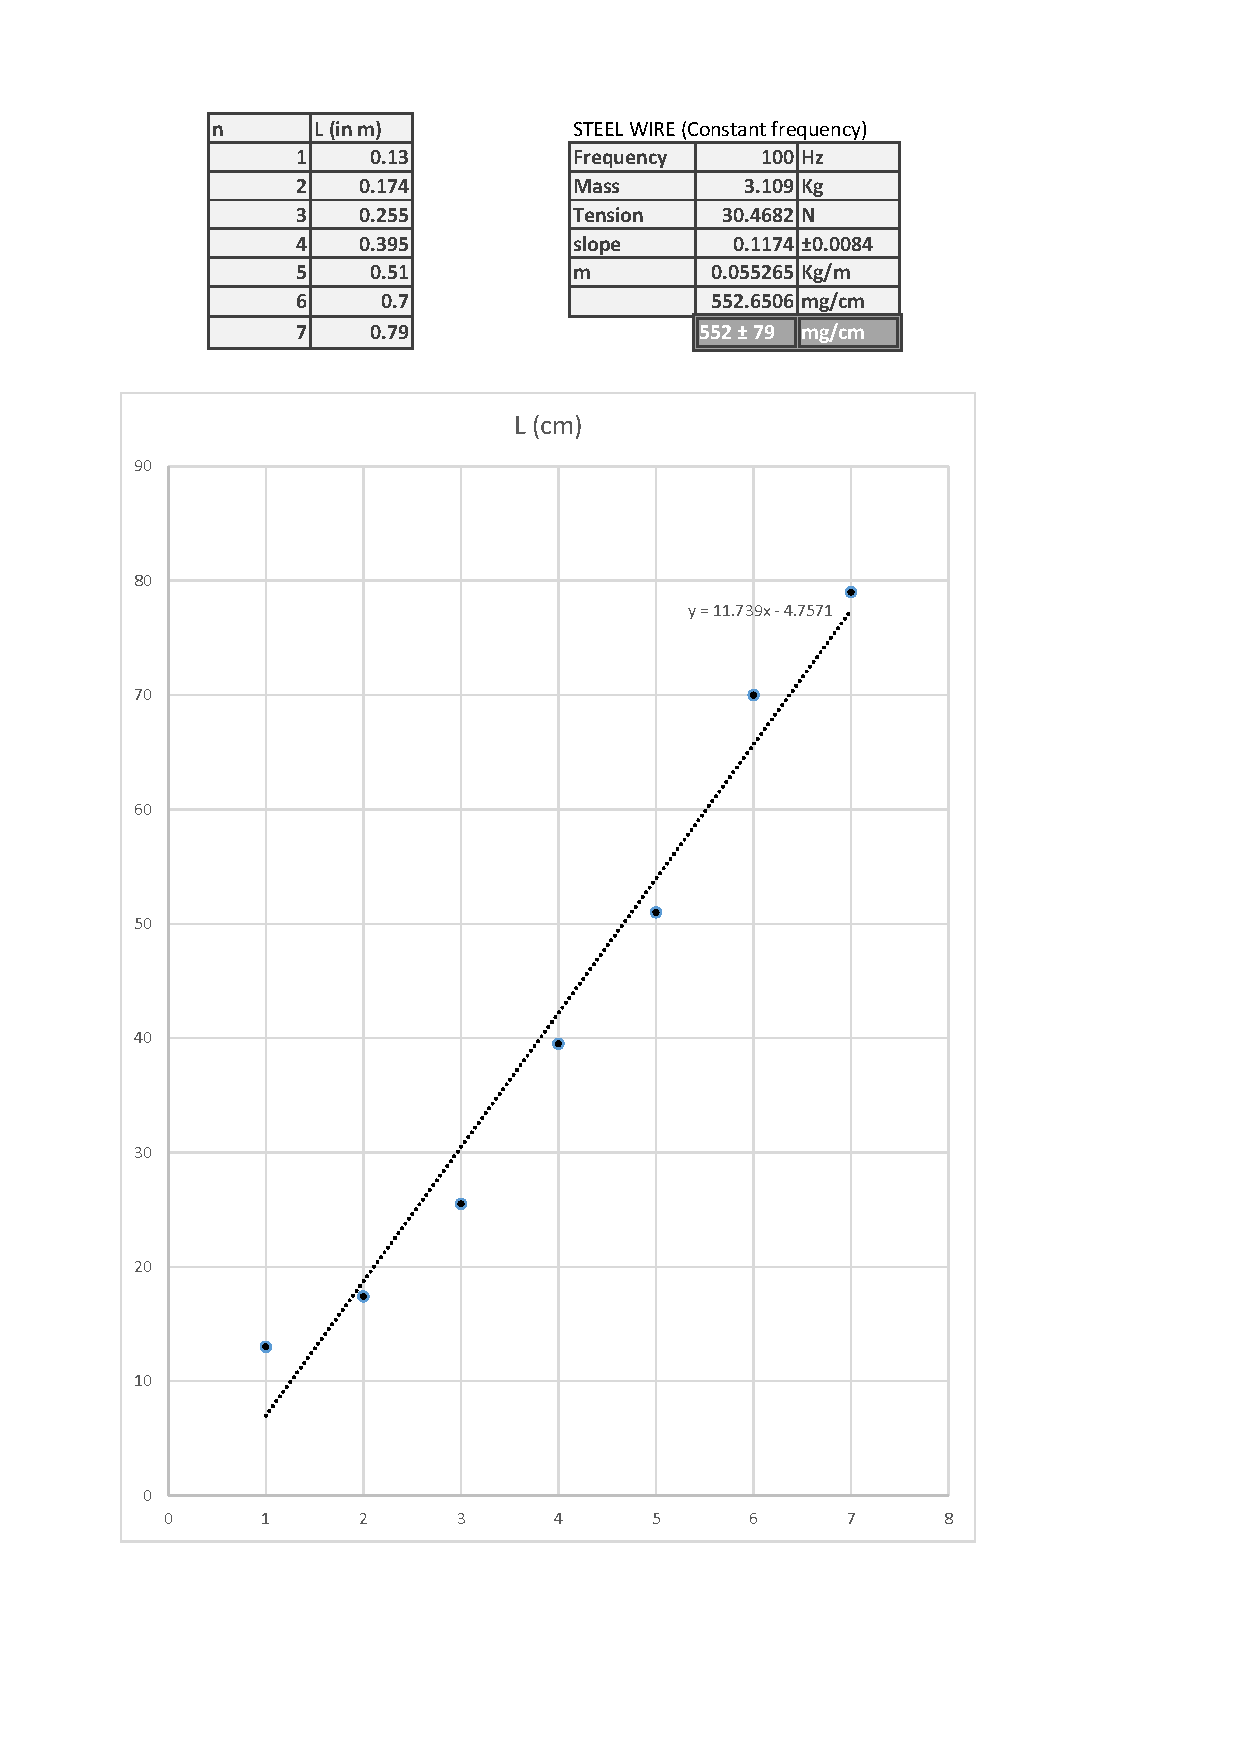
\includegraphics[width=1.3\linewidth]{gfx/steel_2}
		\end{center}
		\caption[Steel Wire (constant AC)]{Steel Wire (constant AC)}
	\label{4_steel2}
	\end{figure}

	
\section{Precautions}
	\begin{enumerate}		
		\item Micrometer should be moved only in one direction to avoid errors due to backlash.
		\item Ensure the table isn't disturbed while taking one particular round of measurements.
		\item Be sure to use the ammeter in the right range for best results.
	\end{enumerate}